\chapter{Capitolo 1}

\section{Definizione di Machine Learning (Arthur Samuel - 1959)}

Il machine learning è un campo di studi che permette ai computer di imparare senza essere esplicitamente programmati.

A differenza degli algoritmi creati finora, un algoritmo di machine learning può imparare come risolvere uno specifico problema di un set di dati. Questo permette di spostare il nostro focus non più a sviluppare tutti gli step necessari affinchè un algoritmo risolvi il problema, ma creare un algoritmo che riesca ad imparare come risolverlo.

\section{Perchè abbiamo bisogno del Machine Learning}

L'approccio utilizzato finora per risolvere i problemi è quello di:

\begin{itemize}
\item Trovare una logica per risolvere il problema
\item Scrivere un programma
\item Suddividerlo in pezzi più piccoli (funzioni)
\item Automatizzare l'approccio
\end{itemize}

Questo funziona per problemi che sappiamo come risolvere ad esempio:

\begin{itemize}
    \item Computare l'area di un poligono
    \item Risolvere equazioni differenziali
\end{itemize}

\noindent
Nel caso del poligono, supponendo di voler calcolare l'area di un rombo i dati presi in input sono dati dalla coppia $(x_1,x_2)$ che rappresentano rispettivamente la diagonale principale e secondaria.
Questi dati verranno passati ad un algoritmo che si occuperà di calcolarne l'area $\frac{x1*x2}{2}$ e generarne un output

\[
\text{input} -> \text{algoritmo} -> \text{output}
\]

Alcuni problemi tuttavia hanno un alto grado di \textbf{incertezza} che rende il problema più difficile da affrontare dovuto al fatto che non siamo in grado di fare assunzioni sui dati che vorremmo vedere e non sempre sappiamo come risolvere determinati task. Come per esempio:

\begin{itemize}
\item Distinguere email spam e non spam
\item Classificare un'immagine per determinare quale oggetto rappresenta
\end{itemize}

\section{Esempio delle email spam e non-spam}

Vogliamo creare un algoritmo di machine learning in grado di determinare se una mail data è spam o meno, la classificheremo quindi come \textbf{spam} altrimenti come \textbf{ham}.

\begin{description}
    \item[Spam:] Email non desiderata, spesso di natura pubblicitaria, inviata in massa a più destinatari.
    \item[Ham:] Email legittima, non spam.
\end{description}

\paragraph{Esempi:}

\begin{itemize}
    \item Compra prodotto a 10\$! Oferta imperdibile! $\rightarrow$ Spam
    \item Ciao Giovanni, come stai? $\rightarrow$ Ham
\end{itemize}

\section{Machine Learning Algorithm (Tom Mitchel - 1998)}

Un algoritmo si dice che apprende dall'\textbf{esperienza E} rispetto a una certa classe di \textbf{Task T} e a una misura di \textbf{performance P}, se la sua \textbf{performance} nel compito \textbf{T}, misurata tramite \textbf{P}, migliora con l’\textbf{esperienza E}.

\section{Definizione di Task}

Rappresenta il problema che deve essere risolto. nell'esempio di determinare se una mail è spam o meno è quello di \textbf{predire} l'etichetta (Y="spam" oppure Y="ham") ed è strettamente legata al modello, funzione parametrizzata, che indichiamo con \textbf{h}.

\section{Definizione di Esperienza}

Rappresentano i dati, ovvero i valori assunti dalle \textbf{random variables}, nell'esempio X è il contenuto della mail ed Y l'etichetta. La coppia di valori:

$$
  {\{(X=x_i, Y=y_i)\}}_{i=1}^N
$$

\noindent
Rappresenta l'esperienza. Generalmente vista come una collezione di elementi chiamati \textbf{esempi}.

\section{Definizione di Performance}

Funzione che valuta quanto bene il computer è in grado di risolvere un certo task T.
Supponiamo che il nostro algoritmo abbia previsto un insieme di etichette per un dato numero di email che indichiamo con:

$$ \{\hat{y_i}\} $$

\noindent
Dove il simbolo 'hat' indica che il dato non è stato osservato ma \textbf{previsto}. L'insieme delle etichette corrette è invece dato da

$$ \{{y_i}\} $$

\noindent
Per valutare la qualità del nostro metodo, dovremmo confrontare i due insiemi di previsioni utilizzando una \textbf{misura di performance:}

$$ P(\{{y_i}\},\{\hat{y_i}\} ) $$

\noindent
Questa funzione restituisce un valore reale appartenente al range [0,1].

\begin{itemize}
\item Un \textbf{valore elevato} indica che le previsioni sono accurate
\item Un \textbf{valore basso} indica che le previsioni non sono accurate.
\end{itemize}

\noindent
Indichiamo con il termine \textbf{misura di errore} il valore: $1 - P$. Per risolvere problemi di machine learning ci affidiamo a modelli statistici che dipendono dal task.

\section{Esempio completo}

Siano:

\begin{itemize}
\item $x^{(1)}$: Il testo dell'email 1: "Compra prodotto a 10\$! Oferta imperdibile!"
\item $x^{(2)}$: Il testo dell'email 2: "Ciao Giovanni, come stai?"

\item $y^{(1)}$: L'etichetta \textbf{spam}
\item $y^{(2)}$: L'etichetta \textbf{ham}
\item h: Il modello
\end{itemize}

\noindent
Allora

$$ h(x^{(1)}) = \hat{y}^{(1)} $$

\noindent
e

$$ h(x^{(2)}) = \hat{y}^{(2)} $$

\section{Task, Esempi ed Etichette}

Un esempio è generalmente espresso come una raccolta di valori che sono stati misurati quantitativamente da un evento osservato. Un esempio è generato da un vettore:

$$ x \in \mathbb{R}^{N} $$

\noindent
Scritto anche come:

$$ x = (x_1, x_2, ..., x_n)$$

I valori del vettore x sono detti \textbf{features} in quanto rappresentano le proprietà specifiche degli esempi in input. Se la dimensionalità di x è 10, diremo che ha 10 features Nella maggior parte dei casi, ogni esempio x è anche abbinato a un output desiderato y. Tali output desiderati sono anche chiamati etichette. Un'attività può quindi essere definita come un certo modo di elaborare un esempio di input per ottenere un output.

Nell'esempio: Determinare se un'e-mail è spam o ham. In questo caso, l'input è l'email, le features possono essere caratteristiche dell'email come il numero di errori ortografici o la presenza di alcune parole chiave, mentre l'output atteso è l'etichetta (spam o ham).

\section{Estrazione delle features}

Per gestire le email, dobbiamo prima trasformarle in un'entità quantificabile. Questo di solito viene fatto identificando alcune caratteristiche dei dati che sono importanti per il compito dato (numero di errori ortografici o la presenza di alcune parole chiave). In pratica, stiamo cercando una funzione f che trasformi l'"entità" dalla sua forma originale a una forma di destinazione, che è buona per risolvere un compito specifico:

$$f(d) = x$$

Dove d è il dato grezzo di input (ad esempio, il messaggio di posta elettronica completo), f è la funzione di trasformazione e x è l'output della trasformazione, che sarà l'input dell'algoritmo di apprendimento automatico.

La funzione f è chiamata \emph{rappresentazione}. L'output della trasformazione x è anche chiamato rappresentazione.
Poiché rappresentando i dati otteniamo un vettore di funzionalità, il processo di rappresentazione dei dati è talvolta chiamato \textbf{features extraction}. Non ci sono «rappresentazioni universali», ma solo rappresentazioni che servono a qualche compito.

\noindent
Le rappresentazioni sono di 2 tipi:

\begin{itemize}
\item Create a mano
\item Apprese
\end{itemize}

\noindent
L'estrazione delle features mette in luce caratteristiche salienti trascurandone altre.

\section{Features}

L'output di una funzione di rappresentazione è quindi in generale un esempio

$$ x = (x_1, x_2, ..., x_n)$$

\noindent
composto da un insieme di features . \textbf{Una feature è la specifica di un attributo.}
Si tratta di una misura che rappresenta aspetti dei dati che è utile evidenziare per risolvere il problema considerato. Ad esempio, il colore può essere un attributo. "Il colore è blu" è una funzionalità estratta da un esempio.

\noindent
Le caratteristiche possono essere di due tipi principali:

\begin{description}
    \item[Categoriche:] un numero finito di valori discreti. Questi possono essere:
    \begin{itemize}
        \item \textbf{Nominali:} a indicare che non esiste alcun ordinamento tra i valori, ad esempio cognomi e colori.
        \item \textbf{Ordinali:} a indicare che esiste un ordinamento, ad esempio in un attributo che assume i valori basso, medio o alto.
    \end{itemize}
    \item[Continue:] comunemente, sottoinsieme di numeri reali, dove c'è una differenza misurabile tra i valori possibili. I numeri interi sono solitamente trattati come continui nei problemi pratici.
\end{description}

\section{Esempio delle Email Spam e Non Spam}

Consideriamo il nostro esempio in cui vogliamo distinguere le e-mail spam da quelle non spam.
L'input del processo sono i messaggi di posta elettronica, quindi dobbiamo trasformarli in vettori di features:

$$ x = (x_1, x_2, ..., x_n)$$

\noindent
con un processo di \emph{features extraction}.

Naturalmente, ci aspettiamo che le funzionalità estratte siano utili per risolvere il nostro compito di determinare se un'e-mail è spam o ham. Possiamo notare che le e-mail di spam spesso includono errori ortografici e parole come "Acquista", "occasione" e "10\$". Quindi, potremmo decidere di rappresentare ogni messaggio di posta elettronica con due numeri:

\begin{itemize}
    \item Il conteggio degli errori ortografici.
    \item Il numero di volte in cui alcune parole o pattern specifici appaiono nel testo.
\end{itemize}

Una volta che i messaggi di input sono stati convertiti in vettori di funzionalità, possono essere visti come vettori nello spazio 2D.

\begin{figure}[htbp]
    \centering
    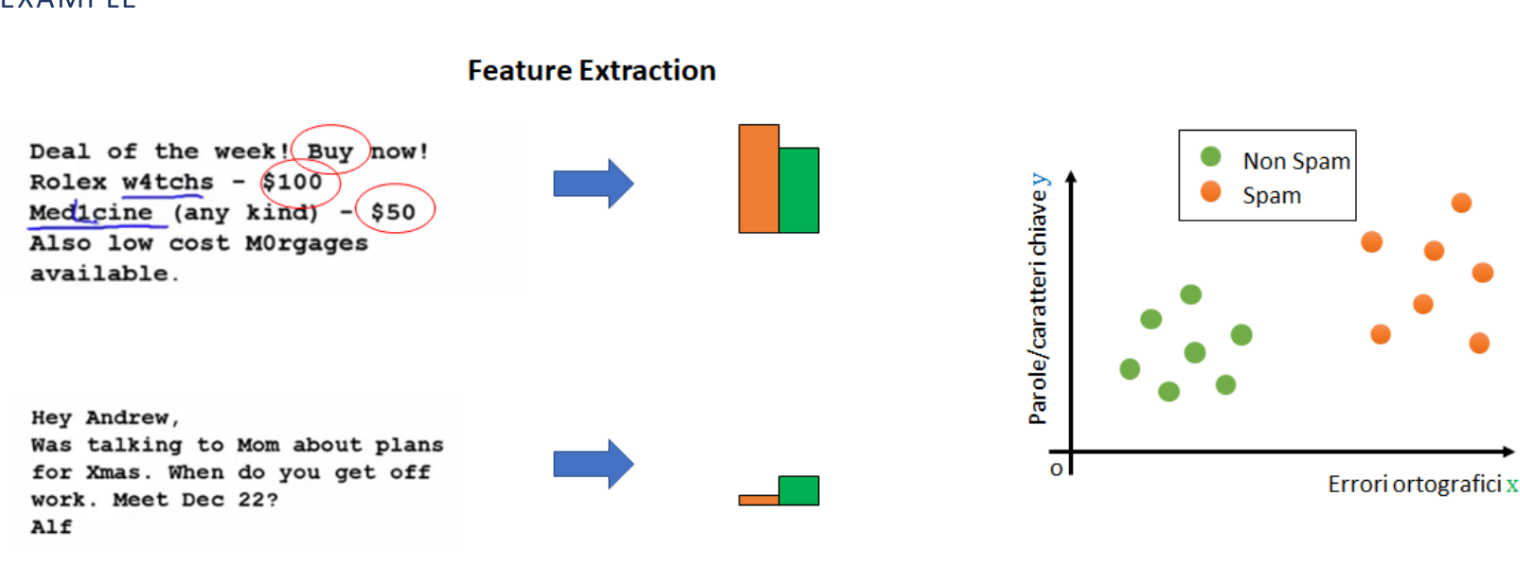
\includegraphics[width=\textwidth]{images/featureExtraction.png}
    \caption{Estrazione delle feature: le e-mail vengono trasformate in vettori 2D, dove $x = \text{errori ortografici e } y = \text{pattern ripetibili}$, e proiettate nello spazio delle feature, , dove la separazione tra spam (arancione) e non spam (verde) risulta evidente.}
    \label{fig:featureExtraction}
\end{figure}

\section{Tipologie di Task}

Le attività possono essere di diversi tipi. Di seguito, discuteremo due compiti principali:

\begin{itemize}
\item Classificazione
\item Regressione
\end{itemize}

Assumeremo che ogni algoritmo di apprendimento automatico prenda come input esempi che sono già stati rappresentati con una funzione di rappresentazione adeguata.

\section{Classificazione}

In questo tipo di attività, alla macchina viene chiesto di specificare a quale di un insieme predefinito di categorie K appartiene l'input.

\noindent
Esempi di questo compito sono:

\begin{itemize}
\item Classificare i post di Facebook come riguardanti la politica o qualcos'altro (classificazione politica vs non politica).
\item Rilevamento delle e-mail di spam (classificazione dello spam vs legittima delle e-mail).
\item Riconoscimento dell'oggetto raffigurato in un'immagine tra 1000 oggetti diversi (riconoscimento dell'oggetto).
\end{itemize}

\noindent
L'algoritmo di apprendimento è solitamente fornito con un insieme di esempi:

$$ \{x^{(1)}, x^{(2)}, ..., x^{(n)}\} \text{ dove: } x^{(j)} \in \mathbb{R}^{N} \forall j$$

\noindent
e un insieme di etichette corrispondenti

$$ \{y^{(1)}, y^{(2)}, ..., y^{(n)}\} \text{ dove: } y^{(j)} \in \{1,..,k\}\forall j$$

\noindent
che specificano a quale delle categorie K appartiene ogni esempio.

Ad esempio, se $y^{(j)} = 3$, allora $x^{(j)} $ appartiene alla classe "3".

Nel caso della classificazione binaria (ad esempio, spam vs non spam), $y^{(j)} \in \{0,1\} $. Per risolvere questo compito, l'algoritmo di apprendimento automatico assume la forma di una funzione:

$$ h: \mathbb{R}^{N} \rightarrow \{1, ... ,K\} $$

\noindent
tale che:

$$y^{(j)} = h(x^{(j)})$$

\noindent
Esempio:

\begin{itemize}
    \item \textbf{Classification Task:} data un'e-mail, classificarla come spam o non spam.
    \item \textbf{Input:} esempi n-dimensionali $ x = (x_1, x_2, ..., x_n)$ contenenti le caratteristiche dell'email, come il numero di errori ortografici e l'occorrenza di parole specifiche.
    \item \textbf{Output:} etichette $y \in \{0,1\}$ che indicano se l'e-mail è legittima o spam.
\end{itemize}

\section{Regressione}

In questo tipo di compito, al programma del computer viene chiesto di prevedere un valore numerico dato un input, tipo:
\begin{itemize}
    \item Prevedere il prezzo delle case date alcune caratteristiche come la città, l'età, la zona, ecc.
    \item Prevedere il valore futuro delle azioni di una società dai valori di altre società o da altre statistiche sul mercato (previsione del mercato azionario).
    \item Conta il numero di auto presenti in un'immagine.
\end{itemize}

\noindent
Analogamente alla classificazione, l'algoritmo viene fornito con esempi di training $x \in \mathbb{R}^{N}$ e con gli output desiderati $y \in \mathbb{R}$. L'algoritmo di apprendimento automatico assume la forma di una funzione $ h: \mathbb{R}^{N} \rightarrow \mathbb{R}$ tale che $y^{(j)} = h(x^{(j)})$.

\noindent
Esempio:

\begin{itemize}
    \item \textbf{Regression task:} Predire il prezzo di una casa in base ai suoi metri quadrati.
    \item \textbf{Input:} Dimensione della casa x (valore scalare)
    \item \textbf{Output:} Prezzo y.
\end{itemize}

\begin{figure}
    \centering
    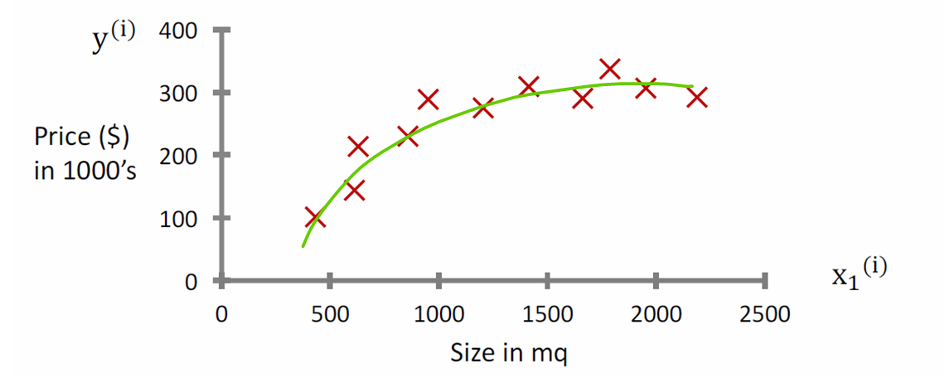
\includegraphics[width=\textwidth]{images/regression.png}
    \caption{Relazione tra dimensione dell’immobile $(x_11^{(i)}$, in mq) e prezzo $(y^{(i)}$, in migliaia di \$): i punti rossi sono i dati osservati, la linea blu rappresenta un modello di regressione lineare che non approssima bene l’andamento non lineare.}
    \label{fig:regressione}
\end{figure}

\section{Supervised Learning e Unsupervised Learning}

Gli approcci di Machine Learning possono essere approssimativamente divisi in supervised e unsupervised learning.

\paragraph{Supervised Learning:} L'algoritmo viene addestrato su un insieme di esempi di input e output desiderati. L'obiettivo è imparare una funzione che mappi gli input agli output corretti.

\paragraph{Unsupervised Learning:} L'algoritmo viene addestrato solo su esempi di input, senza output desiderati. L'obiettivo è scoprire la struttura o i pattern nei dati.

$$ \{x^{(1)}, x^{(2)}, ..., x^{(n)}\} \text{ dove: } x^{(j)} \in \mathbb{R}^{N} \forall j$$

Questi tipi di compiti mirano generalmente a modellare la struttura dei dati. Un esempio di unsupervised learning è il clustering, in cui non viene fornita alcuna informazione aggiuntiva oltre agli esempi.

Gli approcci supervised sono generalmente più facili da gestire, ma richiedono la presenza di labels. Ottenere labels è spesso un problema costoso in termini di tempo, poiché richiede che le persone annotino manualmente i dati. Ad esempio, se dobbiamo costruire un spam-detector utilizzando un approccio supervised, è necessario che qualcuno etichetti manualmente diverse email come ‘spam’ o ‘non-spam’.

\section{Reinforcement Learning}

Alcuni autori fanno riferimento anche a una terza classe di algoritmi di Machine Learning: il Reinforcement Learning.

Il Reinforcement Learning mira a scoprire la soluzione a un problema attraverso il metodo trial and error, piuttosto che tramite istruzioni esplicite su come risolvere il compito. Questo avviene permettendo all'algoritmo di interagire con un environment e ricevere positive rewards quando compie azioni che portano a un buon risultato (rispetto al problema da risolvere) e negative rewards quando compie azioni che portano a un risultato negativo.

L'obiettivo degli algoritmi di Reinforcement Learning è apprendere una policy $\pi$, che possa essere utilizzata per determinare quale azione a intraprendere quando si acquisisce un'osservazione del mondo o. Questo processo ricorda il modo naturale in cui gli animali imparano a risolvere problemi. Ad esempio, si può pensare a un topo che deve trovare l'uscita da un labirinto (immagine \ref{fig:reinforcementLearning}).

\begin{figure}
    \centering
    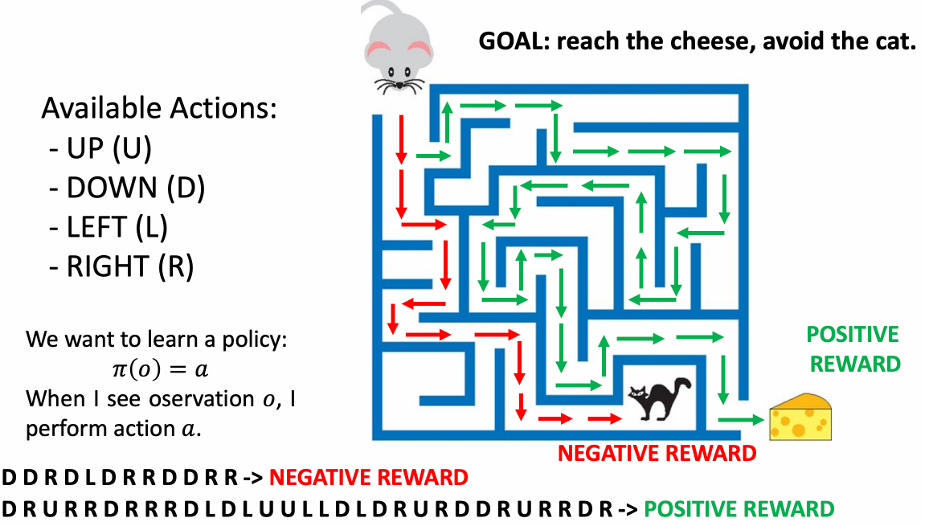
\includegraphics[width=\textwidth]{images/reinforcementLearning.png}
    \caption{Reinforcement Learning nel labirinto: l’agente sceglie tra azioni U/D/L/R e apprende una policy \(\pi(o)=a\) che massimizza la ricompensa, raggiungendo il formaggio (positiva) ed evitando il gatto (negativa).}
\label{fig:reinforcementLearning}
\end{figure}

\section{Misura di Performance (P)}

Per valutare le capacità di un algoritmo di Machine Learning nel risolvere un determinato compito, è necessaria una misura quantitativa delle sue prestazioni. Solitamente, questa performance measure \( P \) è specifica per il task \( T \) che il sistema sta eseguendo.

Per compiti come la classification, spesso si misura la performance utilizzando l'\textbf{accuracy}, ovvero la percentuale di esempi classificati correttamente dal modello. Nel caso della regression, invece, si possono usare altre metriche come il mean squared error.

\noindent
Le misure di performance sono utilizzate per due motivi principali:

\begin{itemize}
\item Capire quando un algoritmo di Machine Learning sta migliorando in un determinato compito.
\item Valutare la performance dell'algoritmo una volta finalizzato.
\end{itemize}

\noindent
Una performance measure può anche essere vista in termini di error. Ad esempio, l'\textbf{accuracy} corrisponde a un error rate (la percentuale di esempi classificati in modo errato), calcolato come \( 1 - accuracy \).

\subsection{Esempio}

Un spam detector analizza cinque email. Le prime tre sono spam, le ultime due non lo sono. L'algoritmo classifica come spam le prime due email e come non spam le ultime tre. In questo caso, la prima e le ultime due classificazioni sono corrette, mentre la terza è errata. La accuracy si calcola come la percentuale di esempi classificati correttamente:

$$
\frac{4}{5} = 0.8 \quad \text{ovvero} \quad 80\%
$$

\section{Experience (E)}

Un algoritmo di Machine Learning apprende dall'\textbf{experience} per migliorare una performance measure su un determinato task.

\noindent
L'\textbf{experience} è costituita da una raccolta di esempi

\[
 \mathbf{x}^{(i)}
\]

\noindent
(noti anche come data points, poiché possono essere mappati in uno spazio multi-dimensionale tramite una funzione di rappresentazione), eventualmente accompagnati dalle relative labels 

\[ y^{(i)} \]

\noindent
(a seconda del task considerato).

\noindent
Esistono due principali tipi di algoritmi di Machine Learning:

\begin{itemize}
\item Supervised approaches (quando abbiamo le paired labels, ad esempio nella classification e nella \textbf{regression}).
\item Unsupervised approaches (quando non abbiamo paired labels, come nel \textbf{clustering}).
\end{itemize}

L'\textbf{experience} assume forme diverse a seconda del tipo di approccio di Machine Learning utilizzato.

\section{Dataset (D)}

Le performance measures vengono generalmente calcolate rispetto a un insieme di esempi, piuttosto che su singoli esempi. Un insieme di esempi (eventualmente con labels) è chiamato \textbf{dataset}. I datasets sono generalmente omogenei, nel senso che i dati contenuti al loro interno hanno un formato simile. Ad esempio:

\begin{itemize}
    \item Nel Fisher’s Iris dataset, tutti gli esempi hanno 4 features e una label corrispondente a una delle tre classi.
    \item In un dataset di immagini di food, ogni immagine è associata a una class che indica il piatto specifico.
\end{itemize}

\section{Design Matrix}

Un modo comune per rappresentare un dataset è utilizzare una design matrix. Poiché ogni esempio è una collezione di \textbf{n} features, un dataset di \textbf{m} elementi può essere rappresentato tramite una matrice

$$ \mathbf{X} \in \mathbb{R}^{m \times n} $$

\noindent
con dimensione m x n.

\begin{itemize}
    \item Ogni riga della design matrix rappresenta un esempio.
    \item Ogni colonna rappresenta una delle features.
\end{itemize}

\noindent
Nel caso del supervised learning, si considera spesso anche un'altra matrice

$$ \mathbf{Y} \in \mathbb{A}^{m \times k} $$

\noindent
dove \( k \) è la dimensionalità degli output desiderati.

\noindent
Ad esempio, nel caso della classification,

\[ \mathbb{A} = \{1, \ldots, M\} \]

\noindent
dove \( M \) è il numero di classi e k è spesso uguale a 1.

\begin{figure}[htbp]
    \centering
    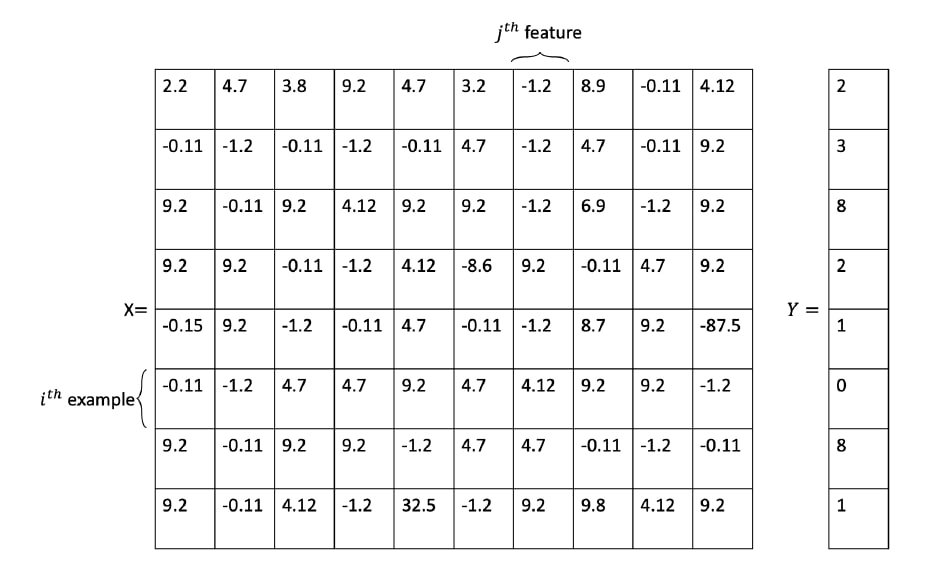
\includegraphics[width=\textwidth]{images/designMatrix.jpg}
    \caption{Design Matrix: rappresentazione di un dataset con m esempi e n features. Ogni riga corrisponde a un esempio, ogni colonna a una feature.}
    \label{fig:designMatrix}
\end{figure}

\subsection{Esempio}

Supponiamo di avere un dataset composto da 1000 email, alcune classificate come spam e altre come not spam. Assumiamo che ogni email sia rappresentata da due features, come discusso nei precedenti esempi.

\noindent
La design matrix che rappresenta il dataset è una matrice

$$ \mathbf{X} \in \mathbb{R}^{1000 \times 2} $$

\begin{itemize}
\item Ogni elemento della matrice rappresenta una delle features di un esempio nel dataset.
\item Ad esempio, $ {X}_{i,1} $ indica il numero di errori ortografici nell’\textbf{i-esima email}, mentre $ {X}_{j,2} $ rappresenta il numero di occorrenze di parole chiave nell’\textbf{j-esima email}, e così via.
\end{itemize}

\noindent
Le labels sono contenute in un vettore

$$ \mathbf{Y} \in \{0,1\}^{1000} $$
dove:

\begin{itemize}
\item $ Y_i $ rappresenta la label associata all’\textbf{i-esimo esempio} (ad esempio, 0 = not spam, \textbf{1 = spam}).
\end{itemize}

\section{Learning}

Un algoritmo di Machine Learning utilizza un dataset di esempi per migliorare la sua performance in un determinato task. Il processo di miglioramento della performance dell'algoritmo è chiamato learning o training.

\subsection{In cosa consiste il training?}

\begin{itemize}
\item Un algoritmo di Machine Learning ha alcuni parametri chiamati parameters, che possono essere regolati per modificarne il comportamento. Questi parametri sono legati a un model (una funzione matematica) utilizzata per risolvere il task.
\item Un algoritmo chiamato training procedure utilizza gli esempi forniti per trovare i valori ottimali per questi parameters.
\item Alcuni parametri non possono essere regolati automaticamente dal training. Questi sono detti hyperparameters e devono essere ottimizzati al di fuori della training procedure, spesso attraverso un metodo trial and error.
\end{itemize}

\subsection{Esempio}

Consideriamo un semplice spam detector che classifica le email come spam o non-spam in base al numero di errori ortografici. 

\noindent
L'algoritmo può essere scritto come segue:

\begin{verbatim}
def classify(x):
    if x > A:
        return 1  # Spam
    else:
        return 0  # Non-spam
\end{verbatim}

\noindent
L'algoritmo dipende da un singolo parametro A. La domanda è: quale valore dovremmo assegnare a A? La \emph{training procedure} permette di trovare un valore adatto per A.
\noindent
Una semplice training procedure consisterebbe nel provare diversi valori per A e registrare le performance dell'algoritmo per ciascun valore di A. Alla fine, possiamo scegliere il valore di A che massimizza la performance measure P.
